\subsection{Módulo genérico de los netElements}
	\label{sec:ACG_net}
	
	El módulo \textit{NetElements} (ver Figura \ref{fig:GeneralSystem}) es el encargado de implementar el reporte del estado de ocupación de las vías. A diferencia de otros módulos centrados en el funcionamiento de mecanismos ferroviarios, que leen el estado del elemento que modelan y envían los comandos necesarios para operarlos; el módulo de \textit{NetElements} solo se ocupa de reportar estados de sólo lectura, la presencia o no de una formación ferroviaria en una vía determinada, sin poder modificar sus valores de ninguna manera.
	
	El ACG utiliza la información otorgada por el RNA para determinar las entradas y salidas cada módulo \textit{NetElements}, e implementa un módulo por cada \textit{NetElement} definido en la red. Cada uno de estos módulos tendrá su propio \textit{NetElement}, leerá su estado (\textit{ocupation}) y recibirá consultas de las rutas que los solicitan (\textit{routeCommands}). A su vez, deberán informar a las rutas que los utilizan cuál es su estado (ocupado o libre, en el puerto \textit{state}) y si se encuentran enclavados (liberados, reservados o enclavados; en el puerto \textit{interlock}). El diagrama de bloques de la máquina de estados finitos con camino de datos diseñado para lograr este objetivo se muestra en la Figura \ref{fig:NET_module}.
	
	\begin{figure}[H]
		\centering
		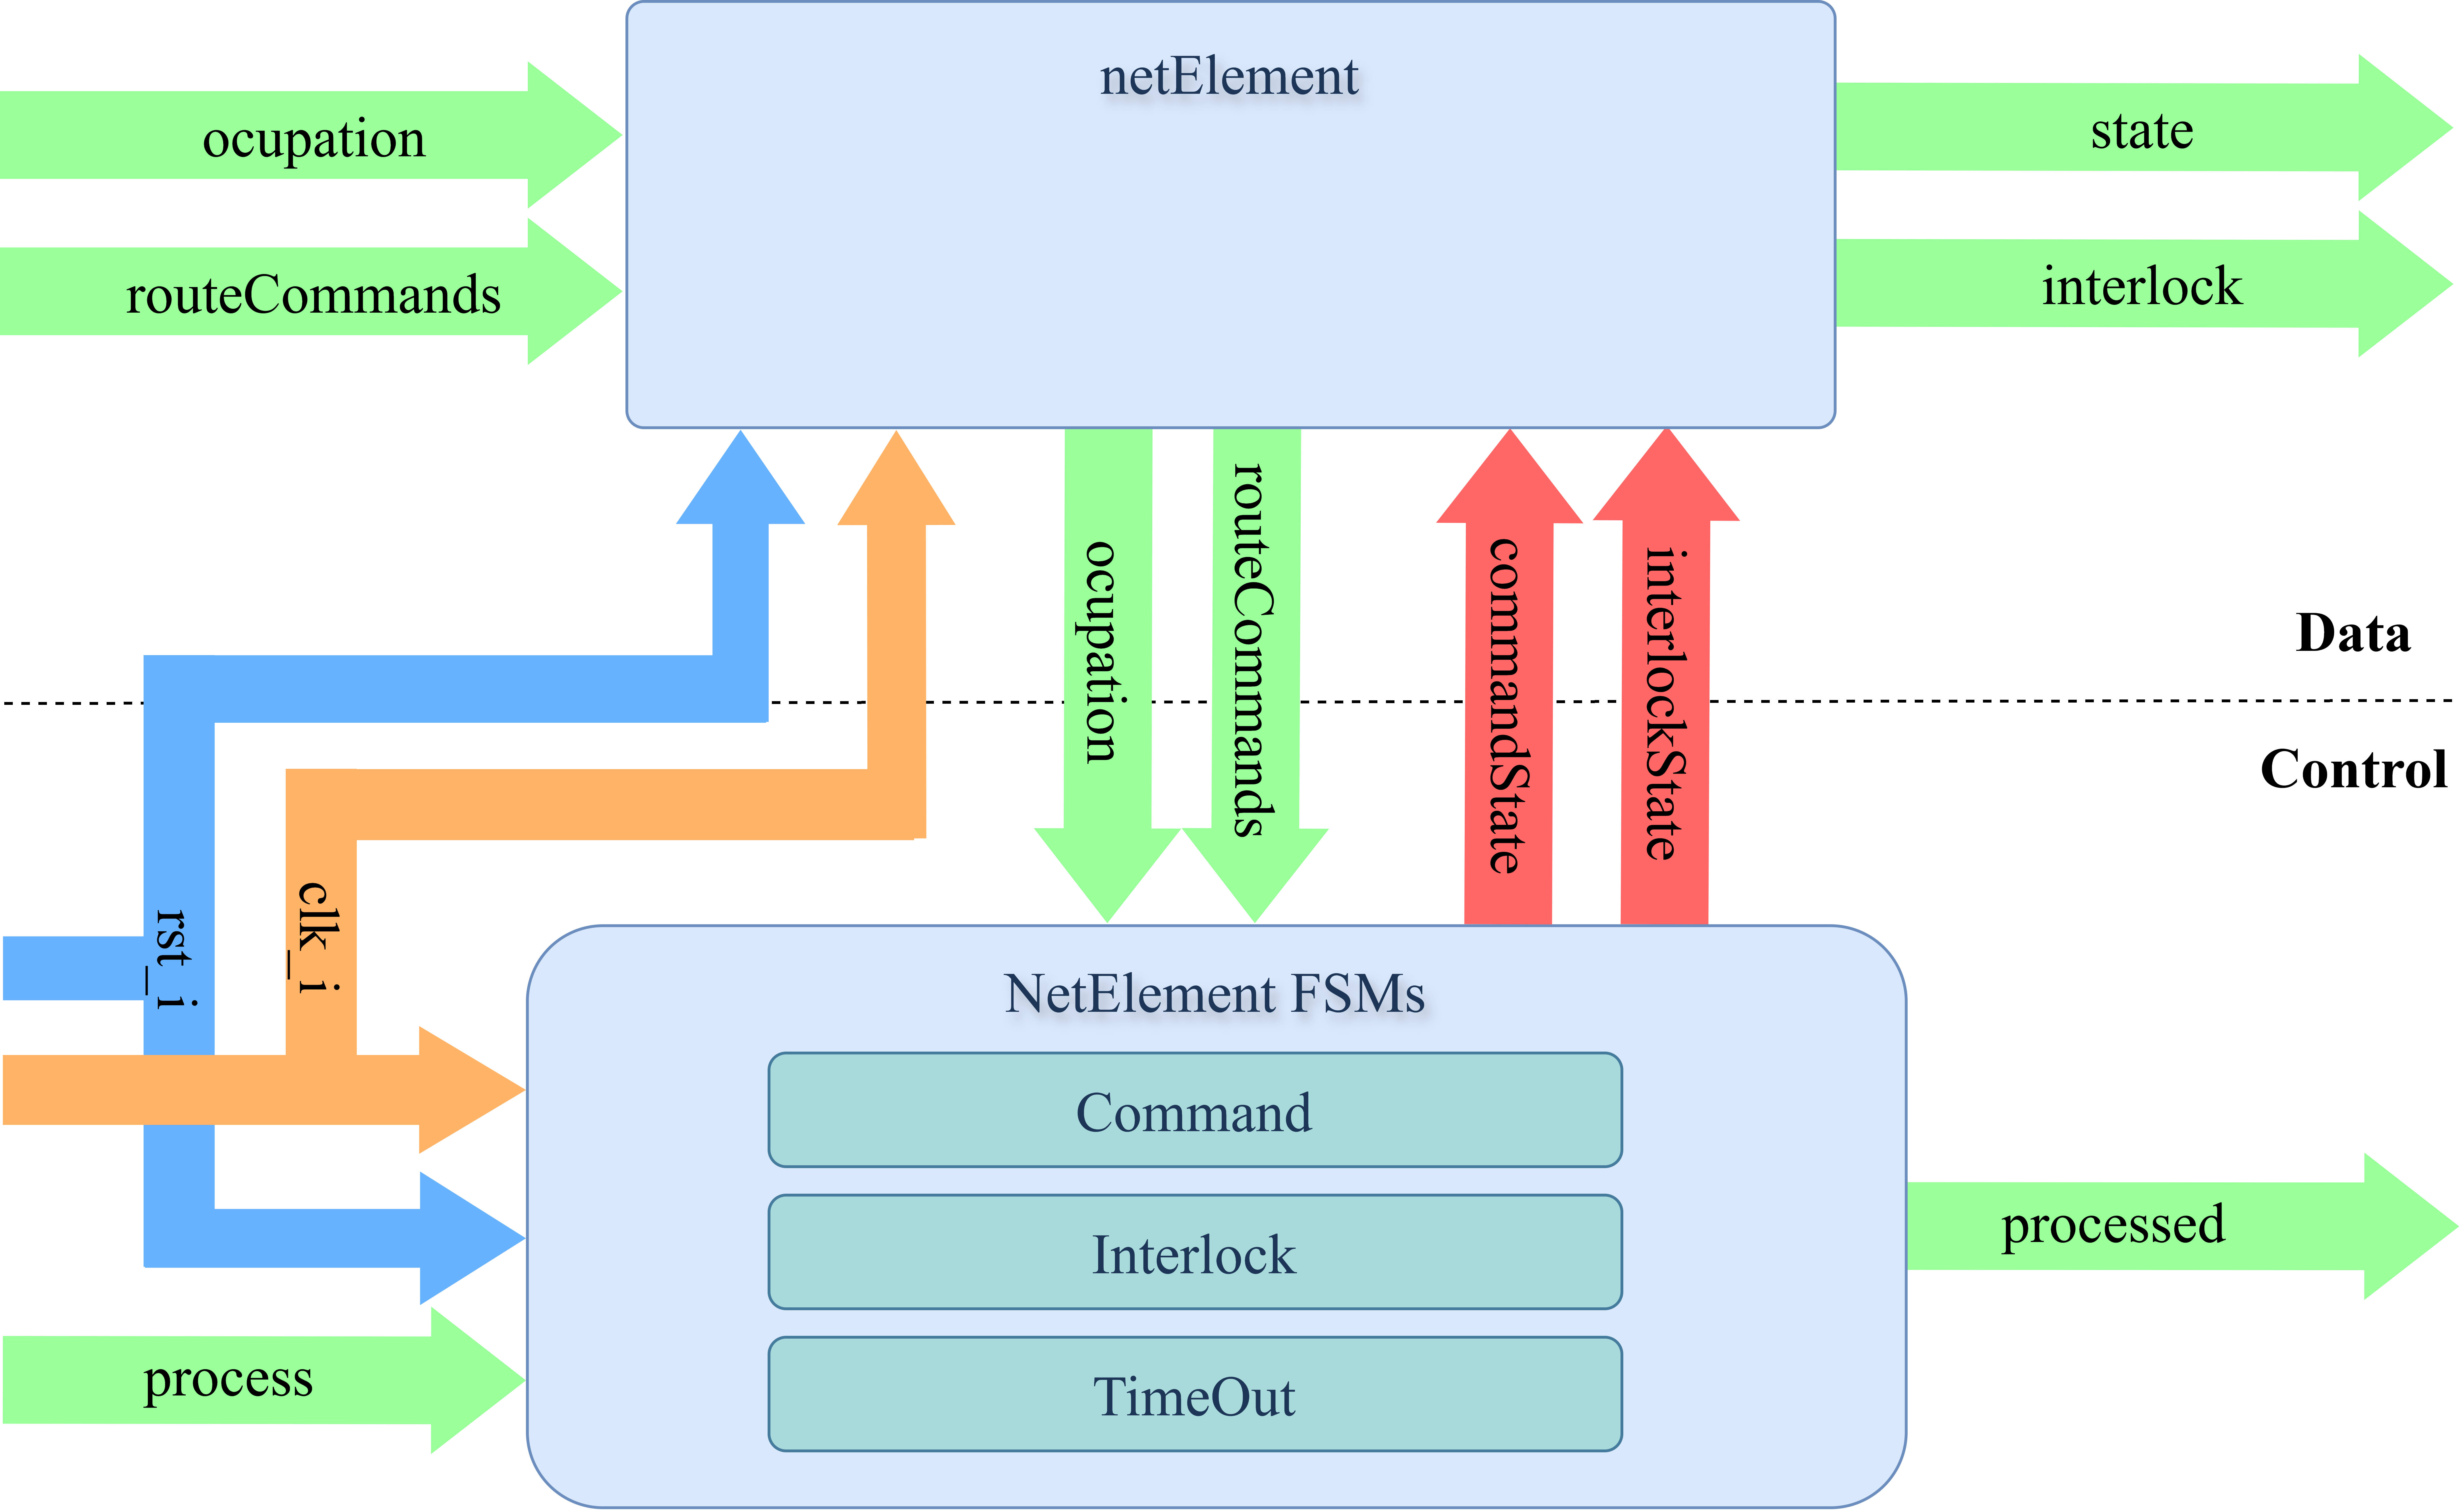
\includegraphics[width=0.8\textwidth]{Figuras/NET_module}
		\centering\caption{FSMD del módulo genérico de \textit{NetElements}.}
		\label{fig:NET_module}
	\end{figure}
	
	Cualquier ruta que pase por sobre el \textit{NetElement} en cuestión puede consultar su estado utilizando el puerto \textit{routeCommands}. Como ya fue explicado en la Sección \ref{sec:detectors}, un circuito de vía asociado a un \textit{netElement} puede estar ocupado por una formación o puede estar libre. Todos los módulos \textit{NetElements} reportaran su estado, independientemente si se encuentran reservados o enclavados. La reserva o enclavamiento es meramente para ser utilizado por las rutas para no considerar como propio un \textit{NetElement} que se encuentra libre pero ya ha sido reservado por otra ruta antagónica. El comportamiento del reporte del estado de ocupación de las vías se define en la red de Petri de la Figura \ref{fig:NET_Petri}.
	
	\begin{figure}[H]
		\centering
		\includegraphics[width=0.6\textwidth]{Figuras/NET_Petri}
		\centering\caption{Red de Petri del modelo dinámico de \textit{NetElements}.}
		\label{fig:NET_Petri}
	\end{figure}
	
	La simpleza de la implementación del módulo \textit{NetElements} facilita una rápida respuesta por parte del sistema de enclavamientos, al otorgar la información requerida solamente a las rutas que la solicitan, lo que reduce enormemente la cantidad de puertos y conexiones a implementar. El ACG crea, además, todas las conexiones necesarias entre cada módulo de elementos ferroviarios y los módulos \textit{NetElements} que los contienen, además de los vecinos mas próximos, para disminuir las chances de que ocurran situaciones peligrosas.